\documentclass[12pt, a4paper]{article}
\usepackage[utf8]{inputenc}
\usepackage{footnote}
\usepackage{hyperref}
\usepackage{fullpage}
\usepackage{amsmath}
\usepackage{pgfplots}
\usepackage{pgfplotstable}
\pgfplotsset{compat=1.8}
\usepackage{cleveref}
\usepackage{graphicx}
\usepackage{tocbibind}
\DeclareMathOperator*{\argmin}{\arg\!\min}
\newcommand{\colvec}[1]{\ensuremath{\begin{pmatrix}#1\end{pmatrix}}}

\begin{document}
\title{Bachelorarbeit\\ zur Erlangung des akademischen Grades\\ Bachelor of Science}
\author{Zachary Schellin\\376930}

\maketitle
\tableofcontents
\section{Introduction}
The Bhatnagar, Gross, Krook equation (BGK) is a kinetic collision model of ionized and neutral gases valid for rarefied as well as other pressure regimes \cite{BGK}. Generating data of such a flow field is essential for various industry and scientific applications[\textbf{REF}]. With the intention to reduce time and cost during the data generating process, experiments were substituted with computational fluid dynamics (CFD) computations. Consequently reduced-order models (ROMs) coupled to aforementioned computations were introduced to further the reduction of time and cost. The thriving field of artificial intelligence appears since the 80's in model order reduction for data visualization/analysis and has now surfaced in fluid mechanics. This thesis will cover the use of artificial intelligence for model order reduction in fluid mechanics.
\subsection{State of the art}
State of the art model reduction of dynamical systems is done via proper orthogonal decomposition (POD) which is an algorithm based on singular value decomposition (SVD)\cite{Franz}\cite{Kutz}. So called POD modes, derived from SVD, describe the principle dynamical behavior of the problem which can be coupled within a Galerkin framework \cite{Franz}. Bernard, Iollo and Riffaud use POD-Galerkin with an additional population of their snapshot database via optimal transport for the proposed BGK equation \cite{Bernard}. Artificial intelligence in the form of autoencoders replacing the POD within a Galerkin framework is evaluated by Kookjin et al. \cite{Carlberg} for advection-dominated problems.
\subsection{Objective of this thesis}
Due to the non-linearity of transport problems in particular shock fronts, the construction of a robust ROM for those cases poses several challenges. Proper orthogonal decomposition (POD) and it's numerous variants like shifted-POD\cite{bibid}, POD-Galerkin\cite{bibid}, POD+I \cite{bibid} to name only a few of them, try to solve this problem by......
\subsection{Thesis outline}
\section{The BGK Equation}
\section{Reduced Order Algorithms}
\subsection{Data Sampling}
\subsection{POD}
The singular value decomposition of the input $X$ [REF to Section 1] gives the optimal low-rank approximation $\tilde{X}$ of $X$ \cref{Eg:eckard-young}[Eckard-Young]. \Cref{Fig:cumu_sing} shows the singular values (left) and the cumulative energy (right) derived from \cref{Eq:cumsum}:
\begin{equation}
S_N = \sum_{k=1}^{N}a_k \qquad\textrm{with a sequence} \qquad\{a_k\}_{k=1}^{n} 
\label{Eq:cumsum}
\end{equation}
\begin{equation}
\underset{\tilde{X}, s.t. rank(\tilde{X})=r}{\operatorname{argmin}} || X -\tilde{X} ||_F=\tilde{U}\tilde{\Sigma}\tilde{V}^*
\label{Eg:eckard-young}
\end{equation}
The first five singular values give an accurate approximation $\tilde{X}$ of $X$.  
As a means to evaluate the low-rank approximation of $X$ we will compare the density derived from \cref{Eq:dense}, computed from $X$ and $\tilde{X}$.
\begin{figure}[htb!]
	\centering
	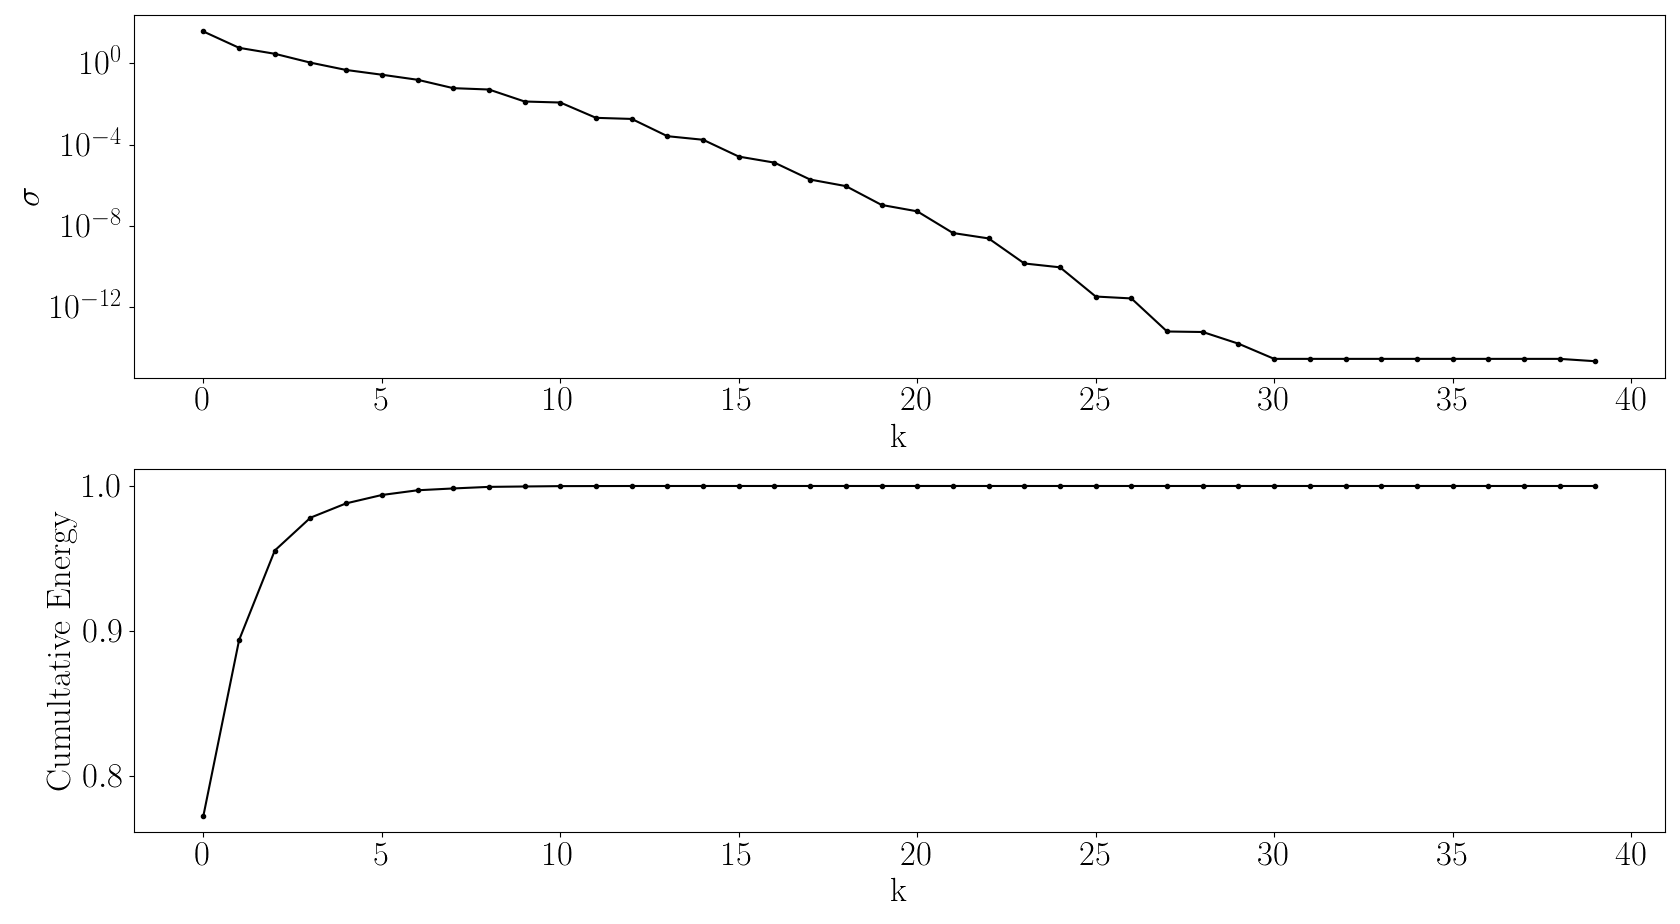
\includegraphics[width=\textwidth]{Figures/Cumultative_Singular_Values_kn001.png}
	\caption{Singular Values (left) and cumultative enrgy (right) over the number of singular values}
	\label{Fig:cumu_sing}
\end{figure}
\subsection{Autoencoders}
The same matrix as in POD is used as input data for the autoencoder:
\[S = \begin{bmatrix}
f(\xi_1,t_1,x_1)&\cdots &f(\xi_n,t_1,x_1) \\
f(\xi_1,t_1,x_2)&\cdots &f(\xi_n,t_1,x_2) \\
f(\xi_1,t_1,x_n)&\cdots &f(\xi_n,t_1,x_n)\\
f(\xi_1,t_2,x_1)&\cdots &f(\xi_n,t_2,x_1)\\
\vdots & \ddots & \vdots\\
f(\xi_1,t_n,x_n)&\cdots &f(\xi_n,t_n,x_n)
\end{bmatrix}\]
During training every 1000 epochs a sample against its prediction was printed in order to link the value of the L1-Loss to a prediction. Using this method a first verification of the model was achieved. Continuing the search for any possible shortage of the models performance, that this method could not cover, eg. samples lying between every 1000 sample, that the model was not able to reconstruct correctly, a second verification process is conducted. 
\section{Results and Latent Manifold Properties}
\subsection{Evaluation Methods}
In oder to evaluate the proposed dimensionality reduction algorithms, two methods are being introduced. The first one constitutes a qualitative analysis using \cref{Eq:sample_dist} which measures the eucledian distance of every reconstructed sample $\tilde{X}_i$ against it`s corresponding original sample $X$.
\begin{equation}
	|X_i-\tilde{X_i}| = \delta_i \qquad\textrm{with i being the i\textsuperscript{th} sample}
	\label{Eq:sample_dist}
\end{equation}
\begin{equation}
	\sum|\rho_i-\tilde{\rho_i}|=\delta_\rho \qquad\textrm{with i being the i\textsuperscript{th} sample}
	\label{Eq:error_rho}
\end{equation}
As a second quantitative approach a comparison of the density over space in time of the BGK model in \cref{Eq:dense} is utilized. The sum over all euclidian distances from the original samples $\rho_i$ to their reconstruction $\tilde{\rho_i}$ is evaluated in \cref{Eq:error_rho}. 
\begin{equation}
\int_{\Re^3}f(\textbf{x},\xi,t)\colvec{1\\\xi\\\frac{||\xi||^2}{2}}d\xi= \colvec{\rho(\textbf{x},t)\\\rho(\textbf{x},t)U(\textbf{x},t)\\E(\textbf{x},t)}
\label{Eq:dense}
\end{equation}
In order to evaluate the performance of the proposed dimensionality reduction algorithms, qualitative and quantitative methods are being introduced. The qualitative analysis comprises a comparision of the sample wise test error following \cref{Eq:sample_dist} on the microscopic data. The Jacobian of the latent code is strongly linked to this measure, as it measures the contraction of the latent manifold. A quantitative measure is taken on the average test error over all over all samples of the microscopic data as well as on the macroscopic data. Both can lead to different conclusions and will be discussed in Section 4.3.
\subsection{Results}
A quantitative measure shows, that the linear Autoencoder performs slightly better than the POD on the input data comparing the density of the original data against the reconstruction. In contrast to this measure, the comparison of the original data to the reconstruction yields the opposite conclusion. 
\begin{center}
\begin{tabular}{ |c|c|c|c| } 
	\hline
	Algorithm & Euclidian distance in Density & Euclidian Distance & Jacobian \\ \hline
	POD & 0.151 & 0.0101 &\\ 
	AE & 0.051 & 0.0102 &\\ 
	CAE 1 & 0.205 & 0.0106 & \\
	CAE 2 & 0.669 & 0.001 & \\
	CAE 2 + tw & 0.385 & 0.0117 & \\
	\hline
\end{tabular}
\end{center}

\begin{figure}[htb!]
	\centering
	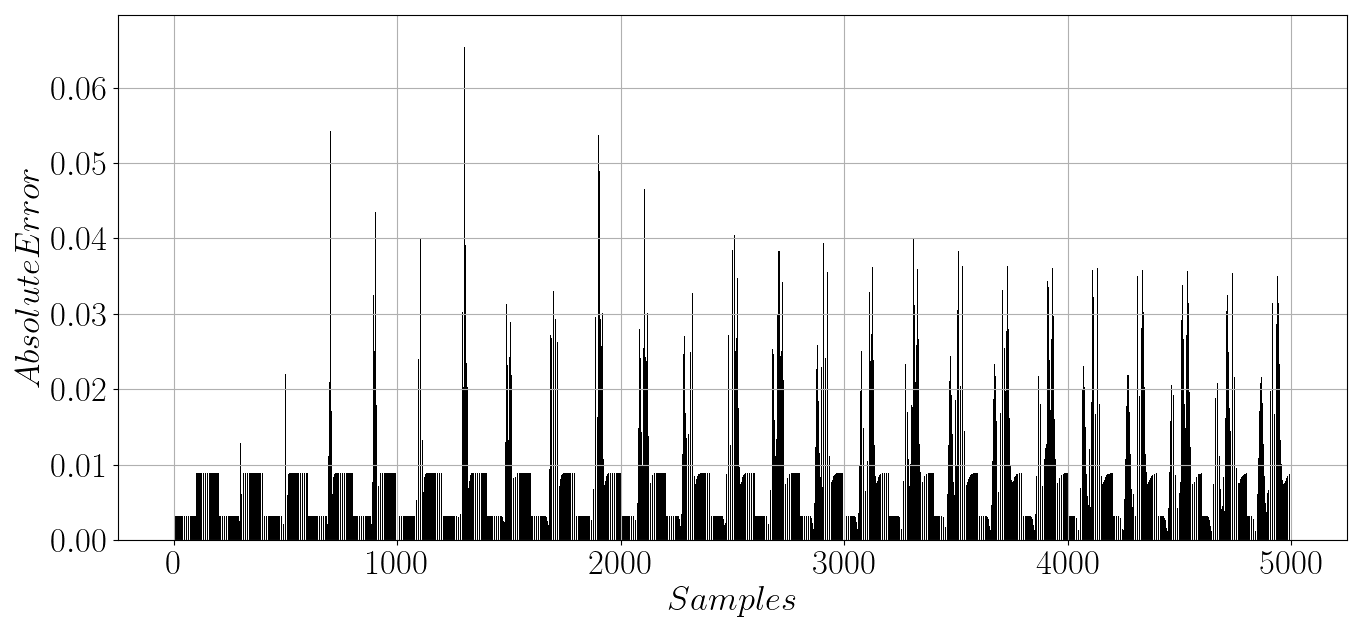
\includegraphics[width=\textwidth]{Figures/Error_samples_SVD.png}
	\caption{Absolute error for every sample in euklidian distance for the POD}
	\label{Fig:Error_samples_svd}
\end{figure}
\begin{figure}[htb!]
	\centering
	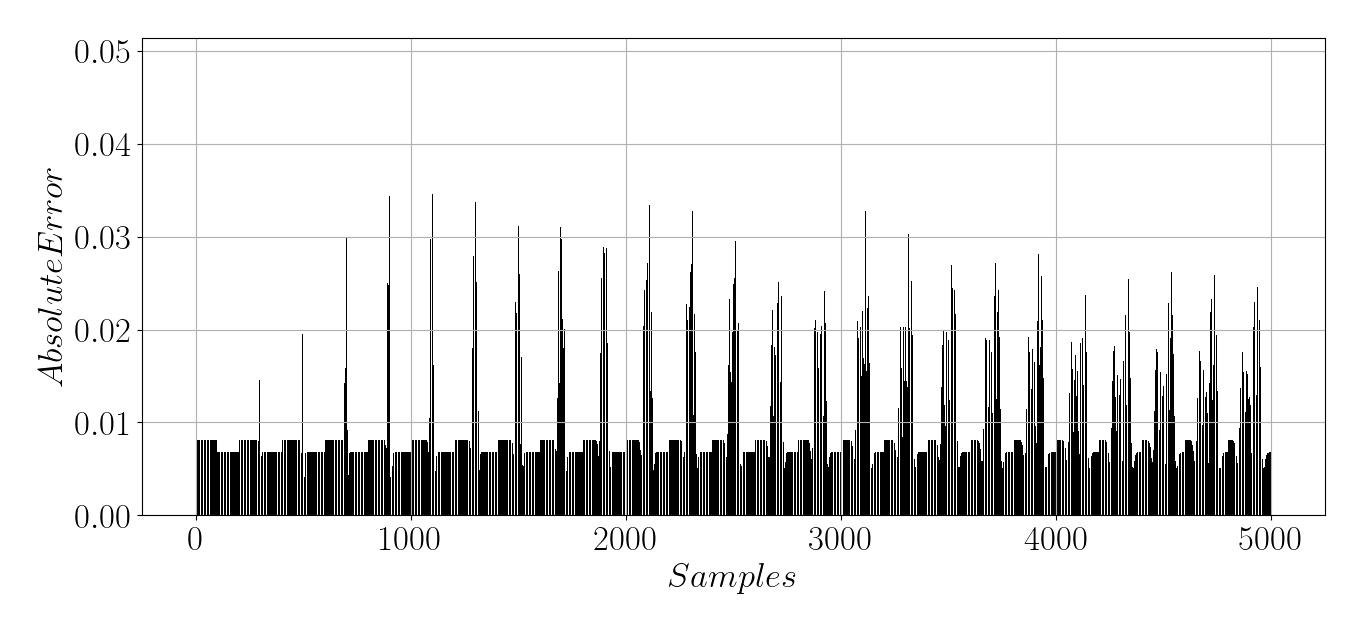
\includegraphics[width=\textwidth]{Figures/Error_samples_v1_1.png}
	\caption{Absolute error for every sample in euklidian distance for the linear autoencoder}
	\label{Fig:error_sample}
\end{figure} 
\begin{figure}[htb!]
	\centering
	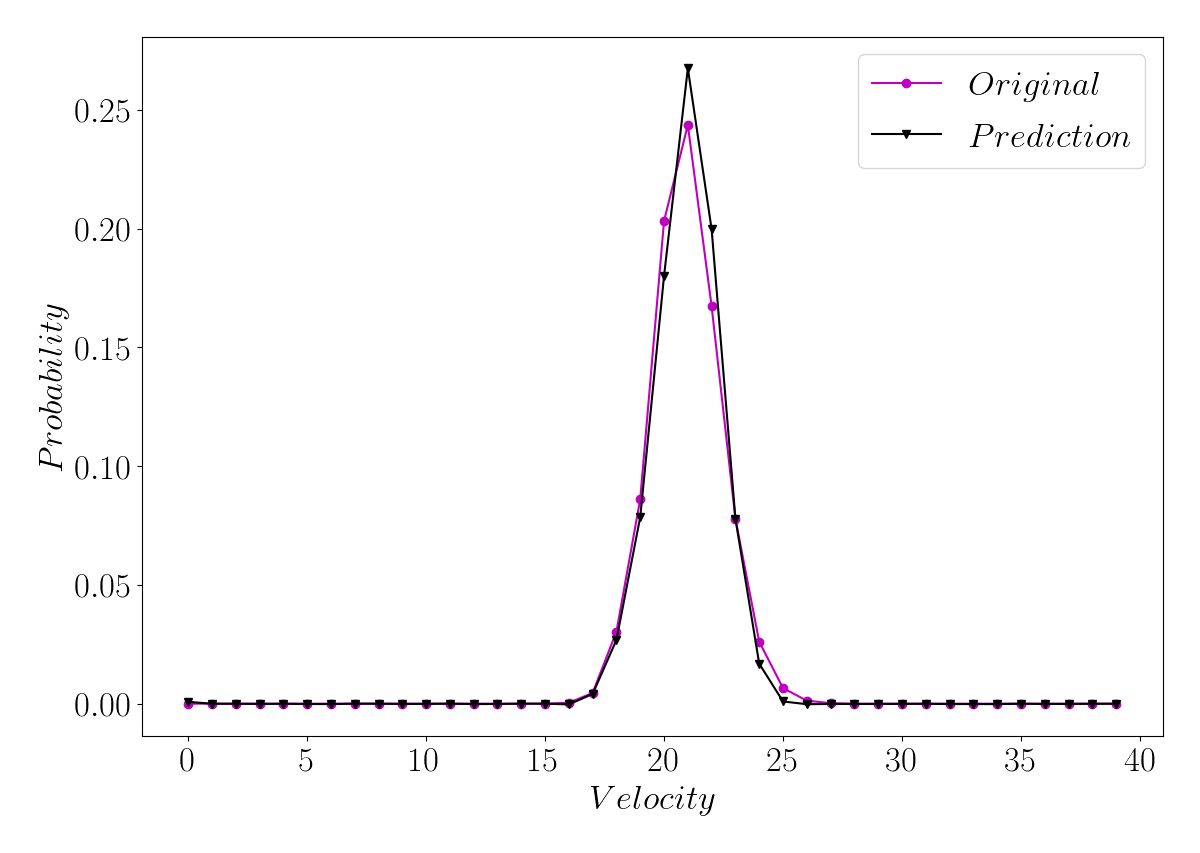
\includegraphics[width=.49\textwidth]{Figures/Sample500_v1_1.png}
	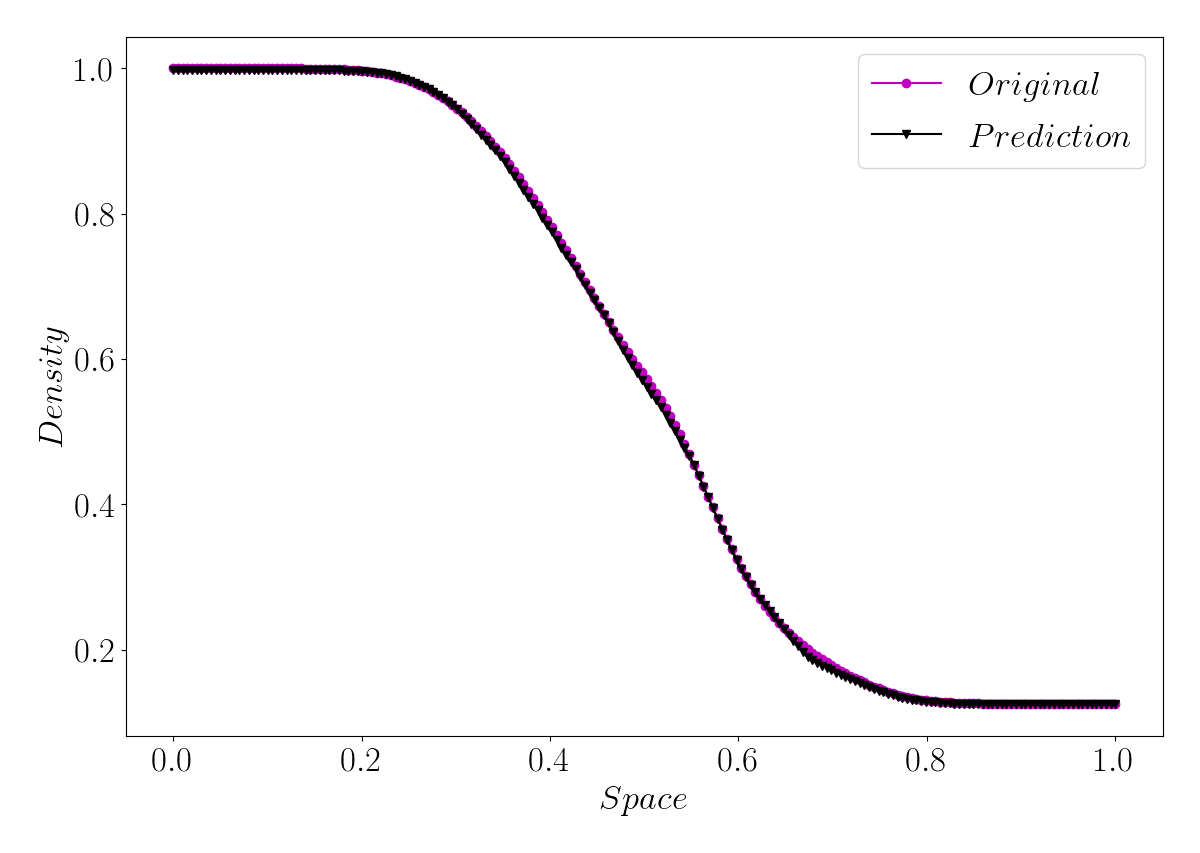
\includegraphics[width=.49\textwidth]{Figures/Density_last_v1_1.png}
	\caption{Error of each sample}
	\label{Fig:Errormore}
\end{figure}
\subsection{Discussion and Outlook}
\bibliography{Bibliography}{}
\bibliographystyle{unsrt}
\end{document}
